\chapter{ Packrat Parsing }
\label{ch:packrat}

Το \textit{Packrat Parsing} \cite{Ford2002a} είναι μία τεχνική για την υλοποίηση συντακτικών αναλυτών για Parsing Expression Grammars.
Ένας συντακτικός αναλυτής packrat, ή αλλιώς packrat parser, προσφέρει την ισχύ και την ευελιξία ενός συντακτικού αναλυτή από πάνω προς τα κάτω με υπαναχώρηση (backtracking) και τη δυνατότητα ανάγνωσης άπειρων προπορευόμενων συμβόλων (infinite lookahead), αλλά εγγυάται γραμμικό χρόνο συντακτικής ανάλυσης.
Οποιαδήποτε γλώσσα ορισμένη από μία LL($k$) ή LR($k$) γραμματική μπορεί να αναγνωριστεί από έναν packrat parser, όπως και άλλες γλώσσες οι οποίες δεν υποστηρίζονται από συμβατικούς γραμμικούς αλγορίθμους συντακτικής ανάλυσης.

Αυτή η επιπλέον ισχύς απλοποιεί: τη διαχείριση των συνηθισμένων συντακτικών ιδιωμάτων, όπως ο κανόνας της μακρύτερης αντιστοίχισης (longest-match rule), επιτρέπει τη χρήση συντακτικών και σημασιολογικών κατηγορημάτων για αποσαφήνιση (disambiguation), παρέχει καλύτερες ιδιότητες για σύνθεση γραμματικών (grammar composition), ενώ δίνει και τη δυνατότητα να ενσωματωθεί η λεκτική ανάλυση στη συντακτική.
Παρόλα αυτά, το packrat parsing θυμίζει την απλότητα και την κομψότητα συντακτικών αναλυτών αναδρομικής κατάβασης.

\section{Θεμέλια}

Ο απλούστερος και διαισθητικά προφανής τρόπος να σχεδιάσουμε έναν συντακτικό αναλυτή είναι η από πάνω προς τα κάτω ανάλυση ή ανάλυση αναδρομικής κατάβασης ή καθοδική συντακτική ανάλυση.
Σε αυτήν, τα στοιχεία της γλώσσας μεταφράζονται σχεδόν άμεσα σε ένα σύνολο από αμοιβαία αναδρομικές συναρτήσεις.
Η καθοδική συντακτική ανάλυση μπορεί να θεωρηθεί ως το πρόβλημα της κατασκευής ενός συντακτικού δέντρου για μια συμβολοσειρά εισόδου, ξεκινώντας από τη ρίζα και δημιουργώντας τους κόμβους του συντακτικού δέντρου με πρωτοδιάταξη (preorder) \cite{Aho2006}. Ισοδύναμα, η καθοδική ανάλυση μπορεί να θεωρηθεί ως η εύρεση ενός αριστερότερου σχηματισμού παραγώγου για τη συμβολοσειρά εισόδου.

Οι καθοδικοί συντακτικοί αναλυτές μπορούν να διακριθούν σε δύο κατηγορίες. Οι \textit{προβλέποντες (predictive) συντακτικοί αναλυτές} επιχειρούν να προβλέψουν ποιο στοιχείο της γλώσσας ακολουθεί, βλέποντας ορισμένα από τα προπορευόμενα σύμβολα στην είσοδο.
Οι \textit{συντακτικοί αναλυτές με οπισθαναχώρηση (backtracking)} παίρνουν αποφάσεις υποθετικά (speculatively) και δοκιμάζουν διαδοχικά διάφορες εναλλακτικές: αν μία αποτύχει, τότε ο αναλυτής οπισθαναχωρεί στη θέση της εισόδου που ήταν προτού δοκιμάσει την εναλλακτική, και μετά εξετάζει την επόμενη εναλλακτική. 

Οι προβλέποντες συντακτικοί αναλυτές είναι γρήγοροι και εγγυώνται γραμμικό χρόνο στην ανάλυση (ως προς το μήκος της εισόδου), ενώ οι αναλυτές με οπισθαναχώρηση είναι πιο απλοί εννοιολογικά αλλά μπορεί να έχουν εκθετικό χρονο εκτέλεσης.

Το packrat parsing αποτελεί μία στρατηγική καθοδικής ανάλυσης που αξιοποιεί τα θετικά και από τις δύο προαναφερθείσες επιλογές. 
Αφενός προσφέρει απλότητα, κομψότητα και γενικότητα όπως ένας αναλυτής με οπισθαναχώρηση, αφετέρου εξοβελίζει τον εκθετικό χρόνο εκτέλεσης, αποθηκεύοντας τα ενδιάμεσα αποτελέσματα από τη συντακτική ανάλυση, ώστε κανένα αποτέλεσμα να μην υπολογιστεί παραπάνω από μία φορά.

Ένας packrat parser μπορεί εύκολα να κατασκευαστεί για οποιαδήποτε γλώσσα που περιγράφεται από μία LL($k$) ή LR($k$) γραμματική, καθώς επίσης και για πολλές γλώσσες που απαιτούν infinite lookahead και δεν είναι, επομένως, LR.
Επιπλέον, είναι πιο εύκολο να κατασκευαστεί από έναν LR αναλυτή (ανοδική ανάλυση), ακόμα και με το χέρι.

\section{Λειτουργία ενός packrat parser}

Είπαμε ότι το packrat parsing συνδυάζει τα πλεονεκτήματα της απλότητας του αναλυτή αναδρομικής κατάβασης με οπισθαναχώρηση και της ταχύτητας του προβλέποντα συντακτικού αναλυτή. 
Αυτό το πετυχαίνει κρατώντας τα ενδιάμεσα αποτελέσματα που υπολογίζει σε έναν \textit{πίνακα υπομνηματισμού (memoisation table)}.

Ο πίνακας αυτός έχει σειρές που αντιστοιχούν σε ένα μη τερματικό της γραμματικής και στήλες που αντιστοιχούν σε μία συγκεκριμένη θέση στην είσοδο. Έτσι, το κελί $(i, j)$ περιέχει το αποτέλεσμα που θα πάρουμε αν προσπαθήσουμε με το μη τερματικό $i$ να αναγνωρίσουμε το κομμάτι της εισόδου που ξεκινάει από τη θέση $j$ και μετά. 
Αυτόν τον πίνακα, μπορούμε είτε να τον γεμίσουμε από πάνω προς τα κάτω, δηλαδή κάνοντας αναδρομική κατάβαση με υπομνηματισμό (memoisation), είτε από κάτω προς τα πάνω, στο πνεύμα του δυναμικού προγραμματισμού.

\subsection{Περιγραφή του συντακτικού αναλυτή με δυναμικό προγραμματισμό}

Στην εκδοχή του δυναμικού προγραμματισμού ξεκινάμε να γεμίζουμε τα κελιά από το δεξί άκρο της εισόδου προς τα αριστερά, και κινούμαστε από τα κατώτερα κελιά στα ανώτερα μέσα σε κάθε στήλη. 
Οποτεδήποτε συμπληρώνουμε ένα κελί, το αποτέλεσμά του αποθηκεύεται και μπορεί να χρησιμοποιηθεί έτοιμο στις κλήσεις άλλων κελιών που δεν έχουν υπολογιστεί ακόμα.

Έστω η γραμματική του Σχήματος \ref{fig:peg_example_def}.

\begin{figure}
	\begin{equation}
		\begin{array}{l}
			Additive \; \leftarrow \; Multitive \; \mlq + \mrq \; Additive \; | \; Multitive \\
			Multitive \; \leftarrow \; Primary \; \mlq * \mrq \; Multitive \; | \; Primary \\
			Primary \; \leftarrow \; \mlq ( \mrq \; Additive \; \mlq ) \mrq \; | \; Decimal \\
			Decimal \; \leftarrow \; \mlq 0 \mrq \; | \; ... \; | \; \mlq 9 \mrq \; 
		\end{array}
	\end{equation}
\caption{Μία PEG γραμματική για αριθμητικές εκφράσεις}
\label{fig:peg_example_def}
\end{figure}

Ο Πίνακας \ref{tab:packrat_dp_example} παρουσιάζει έναν μερικώς συμπληρωμένο πίνακα για είσοδο τη συμβολοσειρά `${2 * (3 + 4)}$'.

\begin{longtable}{lllllllll}
    column & C1 & C2& C3& C4& C5& C6& C7& C8 \\
    \hline
    Additive&  & & $\uparrow$& (7,C7)& X& (4,C7)& X& X \\
    Multitive& &  & \vdots & (3,C5)& X& (4,C7)& X& X \\
    Primary &   & $\leftarrow$ \ldots & \circled{?}& (3,C5)& X& (4,C7)& X& X \\
    Decimal &  & & X& (3,C5)& X& (4,C7)& X& X\\
    \hline
    Input String & '2'& '*' & '('& '3'& '+'& '4'& ')'& EOF\\
	\\

	\caption{Ενδιάμεσα αποτελέσματα  για την είσοδο ${2 * (3 + 4)}$}
    \label{tab:packrat_dp_example}
\end{longtable}

Κάθε στήλη $C_j$ αντιστοιχεί στο σημείο $j$ της εισόδου.
Κάθε γραμμή ($Additive, Multitive$ κλπ) αντιστοιχεί στη συνάρτηση που αναλύει συντακτικά το μη τερματικό $i$.
Για λόγους παρουσίασης, κάθε κελί παρουσιάζεται με δύο τιμές (η υλοποίηση θα είχε διαφορετικές).
Η μία τιμή είναι η σημασιολογική τιμή που επιστρέφεται ως αποτέλεσμα της συντακτικής ανάλυσης.
Η άλλη είναι η στήλη στην οποία θα πάει μετά η ανάλυση, μόλις καταναλώσει μέρος της εισόδου σε εκείνο το κελί.

\newpage

Για παράδειγμα, στη στήλη C4, στη γραμμή Additive, η ερμηνεία είναι η εξής: 
Αν η συνάρτηση που αντιστοιχεί στο Additive, ξεκινήσει την συντακτική ανάλυση από τη θέση 4 (χαρακτήρας `3'), θα καταναλώσει 3 χαρακτήρες (την παράσταση `$3+4$') και θα φτάσει μέχρι το σημείο 7 της εισόδου. 
Η σημασιολογική τιμή που θα επιστραφεί είναι το αποτέλεσμα της έκφρασης, δηλαδή το 7.

Το επόμενο κελί που θα πρέπει να υπολογιστεί είναι το Primary στη στήλη C3.
Για να δείξουμε ένα παράδειγμα του πώς επαναχρησιμοποιούνται τα αποτελέσματα, εστιάζουμε σε αυτό το κελί.

Ο κανόνας για το Primary έχει δύο εναλλακτικές: 
μία έκφραση για το Additive μέσα σε παρενθέσεις ή ένα Decimal.
Αν προσπαθήσουμε τις εναλλακτικές με τη σειρά που δίνονται στη γραμματική, το Primary πρώτα θα ελέγξει για Additive ανάμεσα σε παρενθέσεις.
Για να γίνει αυτό, πρώτα αντιστοιχίζει την αριστερή παρένθεση στη στήλη C3, το οποίο πετυχαίνει, και επιστρέφει την υπόλοιπη συμβολοσειρά η οποία ξεκινάει στη στήλη C4, δηλαδή την `$3+4)$'.
Στην έκδοση του αναλυτή αναδρομικής κατάβασης με οπισθαναχώρηση, το Primary θα έπρεπε να καλέσει αναδρομικά τη συνάρτηση Additive στην εναπομείνασα συμβολοσειρά. 
Ωστόσο, επειδή έχουμε αποθηκεύσει τα ενδιάμεσα αποτελέσματα στον πίνακα, μπορούμε απλά να κοιτάξουμε το αποτέλεσμα της κλήσης Additive στη στήλη C4, που είναι $(7,C7)$. 

Οπότε, η σημασιολογική τιμή είναι το 7 και η νέα θέση που εξετάζουμε στη συμβολοσειρά ξεκινάει στη στήλη C7, όπου βρίσκεται η δεξιά παρένθεση.
Εφόσον, η υποέκφραση της γραμματικής έχει και αυτή το μη τερματικό `)', ο κανόνας πετυχαίνει στη θέση C7, καταναλώνει την παρένθεση και αφήνει το υπόλοιπο στη θέση C8.
Τελικά, το αποτέλεσμα για το Primary στη θέση C3 είναι $(7, C8)$.

Το μέγεθος του πίνακα μεγαλώνει με το μήκος της συμβολοσειράς εισόδου αλλά μόνο γραμμικά, υποθέτοντας ότι η γραμμτική έχει πεπερασμένο αριθμό από μη τερματικά σύμβολα.
Επιπλέον, θεωρώντας ότι η γραμματική είναι εκφρασμένη σε Backus-Naur Normal Form, μόνο ένας συγκεκριμένος αριθμός από ενδιάμεσα αποτελέσματα χρειάζεται να προσπελαστεί για να υπολογιστεί ένα νέο αποτέλεσμα.
Επομένως, υποθέτοντας ότι η προσπέλαση ενός κελιού παίρνει σταθερό χρόνο (π.χ. για υλοποίηση με δισδιάστατο πίνακα), η όλη διαδικασία είναι γραμμική ως προς το μήκος της εισόδου.

Ακριβώς επειδή κάθε κελί έχει έναν "δείκτη" προς την επόμενη θέση της εισόδου που θα συνεχιστεί η συντακτική ανάλυση, μπορεί να συμβουλευτεί κελιά που βρίσκονται αυθαίρετα μακριά στον πίνακα.
Για παράδειγμα, ο υπολογισμός του κελιού $[Primary, C3]$ χρειάστηκε αποτελέσματα από τις στήλες C3, C4 και C7. 
Αυτή η ικανότητα να προσπερνάει προπορευόμενα σύμβολα στην είσοδο είναι που του δίνει το infinite lookahead και τον κάνει πιο ισχυρό από έναν LR αναλυτή γραμμικού χρόνου.

\subsection{Περιγραφή του Packrat Parser}

Ένα προφανές πρακτικό πρόβλημα της προσέγγισης με το δυναμικό προγραμματισμό, όπου τα κελιά υπολογίζονται όλα από δεξιά προς τα αριστερά και από κάτω προς τα πάνω, είναι ο υπολογισμός πολλών ενδιάμεσων αποτελεσμάτων που δεν θα χρειαστούν. 
Μία επιπλέον δυσχέρεια είναι πως πρέπει εκ των προτέρων να καθορίσουμε τη σειρά με την οποία θα υπολογιστούν τα κελιά μιας στήλης.
Εμείς είπαμε ότι υπολογίζονται από κάτω προς τα πάνω, όμως αυτό προϋποθέτει εξ αρχής να έχουμε βάλει τη σειρά των μη τερματικών με τέτοιο τρόπο, ώστε τα κάτω κελιά που υπολογίζονται πρώτα, να μην εξαρτώνται από τα πάνω.
Για παράδειγμα, στο Σχήμα \ref{fig:peg_example_def}, οι κανόνες τοποθετήθηκαν έτσι ώστε παρουσιάζουν εξάρτηση από πάνω προς τα κάτω.

To packrat parsing είναι πρακτικά ένας αναδρομικός αλγόριθμος με υπομνηματισμό που λύνει και τα δύο προβλήματα.
Ένας packrat parser υπολογίζει αποτελέσματα μόνο όταν χρειάζονται, με την ίδια σειρά που θα ακολουθούσε και ένας αναλυτής αναδρομικής κατάβασης με οπισθαναχώρηση.
Όμως, άπαξ και ένα ενδιάμεσο αποτέλεσμα υπολογιστεί, αποθηκεύεται για μελλοντική χρήση.

Το Σχήμα \ref{fig:packrat_memo_example} παρουσιάζει τη δομή δεδομένων που δημιουργείται μετά από packrat parsing στην είσοδο `$2 * (3 + 4)$', χρησιμοποιώντας μία εννοιολογική αναπαράσταση με δείκτες που αναπαριστούν τη σχέση μεταξύ των κελιών.
Τα γκρίζα κουτιά που περιέχουν τιμές στην πραγματικότητα δεν θα υπολογιστούν καθόλου.
Τελικά, το μόνο που μας ενδιαφέρει να υπολογιστεί είναι το κελί στη γραμμή που αντιστοιχεί στο αρχικό σύμβολο της γραμματικής ($Additive$) και στη στήλη που αντιστοιχεί στην αρχή της εισόδου (χαρακτήρας `$2$').

\begin{figure}[h]
    \centering
	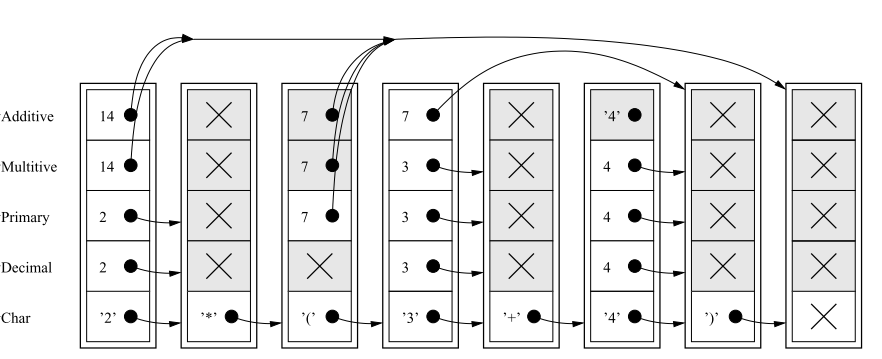
\includegraphics[width=0.70\textwidth]{pics/packrat_memo_example}
	\caption{Παράδειγμα εκτέλεσης Packrat Parsing}
    \label{fig:packrat_memo_example}
\end{figure}

Η αναπαράσταση καθιστά σαφές γιατί ο αλγόριθμος είναι πολυπλοκότητας $O(n)$ ως προς το μήκος $n$ της εισόδου.
Η πρώτη συνάρτηση είναι αυτή η οποία ξεκινά τις αναδρομικές κλήσεις προς άλλες συναρτήσεις.
Κάθε κελί υπολογίζεται το πολύ μία φορά, οπότε ο αλγόριθμος είναι γραμμικός ως προς την είσοδο. 
Προφανώς, η σειρά με την οποία υπολογίζονται τα ενδιάμεσα αποτελέσματα διαφέρει από τον προηγούμενο αλγόριθμο δυναμικού προγραμματισμού, που αναφέραμε νωρίτερα.

\subsection{Ενσωματωμένη λεκτική ανάλυση}

Στους παραδοσιακούς συντακτικούς αναλυτές συνήθως ακολουθείται η παραδοχή ότι η είσοδος έχει ήδη υποστεί προεπεξεργασία από έναν λεκτικό αναλυτή.
Η λεκτική ανάλυση, δηλαδή, είναι ξεχωριστή διαδικασία η οποία χωρίζει τη συμβολοσειρά εισόδου, μετατρέποντάς τη σε ένα ρεύμα (stream) από διακριτές μονάδες (tokens).
O συντακτικός αναλυτής αντιμετωπίζει αυτές τις μονάδες σαν έτοιμα τερματικά, παρόλο που μπορεί να αντιπροσωπεύουν παραπάνω από έναν χαρακτήρες.
Αυτός ο διαχωρισμός προσφέρει αρκετά πλεονεκτήματα όπως ευκολότερη αποσφαλμάτωση ή ευκολότερη ερμηνεία των κανόνων της γραμματικής χρησιμοποιώντας μη τερματικά "υψηλότερου επιπέδου" από απλούς χαρακτήρες.

Στο packrat parsing, το άπειρο lookahead που προκύπτει από την αποθήκευση όλων των ενδιάμεσων αποτελεσμάτων, επιτρέπει άνετα την ενσωμάτωση της λεκτικής ανάλυσης στη συντακτική.
Αρκεί, απλώς, να προστεθούν επιπλέον κανόνες στη γραμματική οι οποίοι θα είναι υπεύθυνοι για τη λεκτική ανάλυση.
Για παράδειγμα, στο Σχήμα \ref{fig:integrated_lex} η εντολή if στην Java, αφενός ορίζεται στη σύνταξη της γλώσσας ως ένα statement που ξεκινάει με τη λεκτική μονάδα "if", αφετέρου η μονάδα αυτή ορίζεται ως ακολουθία δύο χαρακτήρων και, ίσως μετά, κενών χαρακτήρων.

\begin{figure}[h]
\begin{Verbatim}

# Syntax Description
Statement
    <- Block
    / ASSERT Expression (COLON Expression)? SEMI
				...
    / IF ParExpression Statement (ELSE Statement)?

# Token Description
IF <- 'i' 'f' !LetterOrDigit Spacing? 
\end{Verbatim}
\caption{Ενσωματωμένη λεκτική ανάλυση για την εντολή if στην Java}
\label{fig:integrated_lex}
\end{figure}

Έτσι, έχουμε συμπεριλάβει τόσο τη λεκτική, όσο και τη συντακτική ανάλυση της εντολής.

\section{Υλοποίηση}

\subsection{Υλοποίηση της γραμματικής}
Το packrat parsing είναι θεμελιωδώς μία στρατηγική καθοδικής συντακτικής ανάλυσης, οπότε η υλοποίηση του σχετίζεται στενά με τους αναλυτές αναδρομικής κατάβασης. 
Θεμελιώδη ρόλο στην υλοποίηση και στους μετέπειτα πειραματισμούς μας παίζει και ο τρόπος με τον οποίο θα μοντελοποιήσουμε τον αναλυτή αλλά και όλη τη διαδικασία της ανάλυσης, ώστε να αποτυπωθούν σε κώδικα. 
Σε μία γλώσσα αντικειμενοστραφούς προγραμματισμού, όπως η C++, ένας τέτοιος αναλυτής θα μπορούσε να αναπαρασταθεί με ένα αντικείμενο. Το ίδιο και τα διάφορα επιμέρους κομμάτια που αποτελούν την εκάστοτε γραμματική. 

Για καλύτερη οπτικοποίηση και κατανόηση, παραθέτουμε τα UML διαγράμματα που απεικονίζουν την αναπαράσταση των στοιχείων μίας PEG, με βάση τα όσα περιγράψαμε στη θεωρία που προηγήθηκε. Θεωρούμε ότι τα UML διαγράμματα παρουσιάζουν μια απλοποιημένη C++ σύνταξη.

\begin{figure}[h]
    \centering
	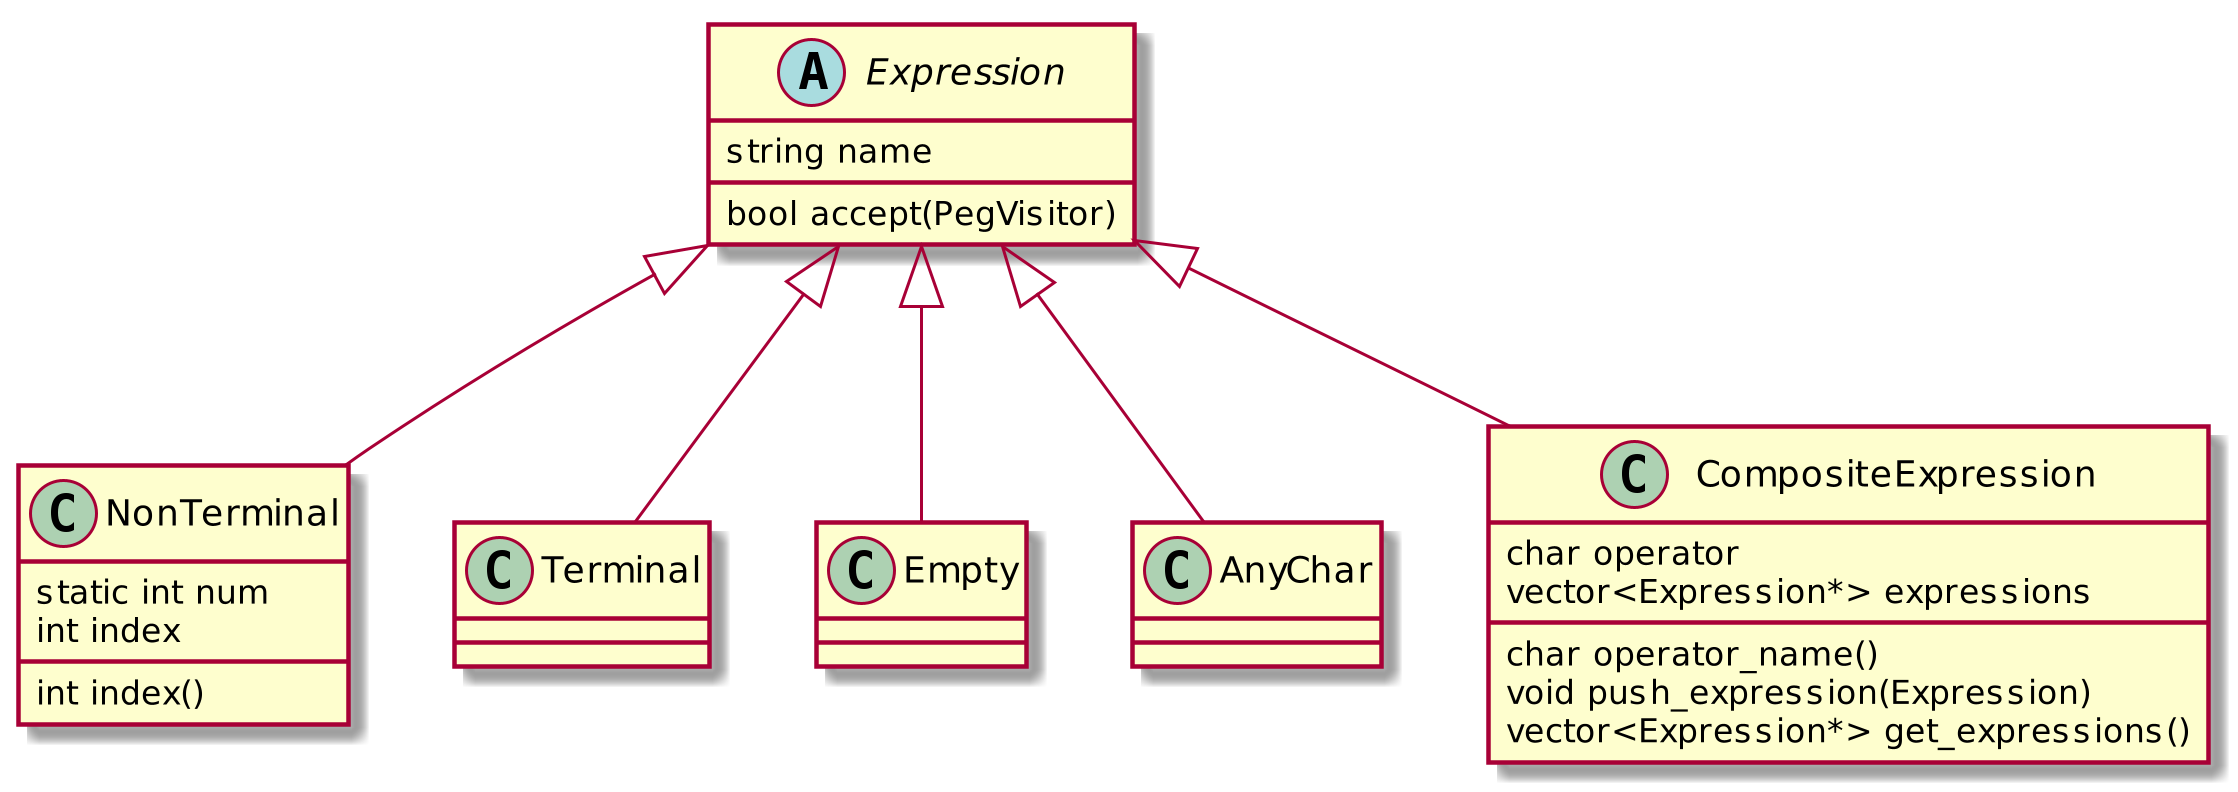
\includegraphics[width=1.10\textwidth]{uml/peg_elements}
	\caption{Μοντελοποίηση των δομικών στοιχείων μίας PEG}
    \label{fig:peg_elements}
\end{figure}

Όλες οι δομικές μονάδες της γραμματικής (τερματικά, μη τερματικά και οι σύνθετες εκφράσεις που τα περιέχουν) είναι εκφράσεις. 
Έτσι, προκύπτουν οι κλάσεις NonTerminal, Terminal και CompositeExpression που κληρονομούν την αφηρημένη κλάση Expression.
Επιπλέον, χρειαζόμαστε και μία έκφραση που να αναπαριστά την κενή συμβολοσειρά (Empty), καθώς και μία που να αναπαριστά οποιονδήποτε χαρακτήρα (AnyChar).
Κατ' ελάχιστο, όλες οι εκφράσεις πρέπει να έχουν ένα όνομα, καθώς και να "δέχονται" έναν "επισκέπτη" (visitor pattern).
Όπως θα δούμε, ο επισκέπτης αυτός είναι ο συντακτικός αναλυτής που θα προσπαθήσει να τις αναγνωρίσει.

Επιπλέον, κάθε μη τερματικό θεωρούμε ότι αντιστοιχεί σε έναν μοναδικό ακέραιο index. 
Ακόμη, το CompositeExpression θεωρούμε ότι αποτελεί το σύνολο των Expressions που συνδέονται με έναν μόνο τελεστή. 
Για παράδειγμα:

\begin{equation}
	A / (B C)
\end{equation}

Εδώ υπάρχει ένα CompositeExpression (έστω $C_1$) με τελεστή την ακολουθία και εκφράσεις τα $B$ και $C$, καθώς και ένα CompositeExpression με τελεστή την διατεταγμένη επιλογή (`$/$') και εκφράσεις τα $A$ και $C_1$. 
Στο Σχήμα \ref{fig:peg_elements} φαίνονται ενδεικτικά οι βασικές μέθοδοι των κλάσεων με βάση τα πεδία που περιγράψαμε.

Με βάση αυτές τις δομικές μονάδες κατασκευάζουμε την κλάση μίας γραμματικής PEG, όπως φαίνεται στο Σχήμα \ref{fig:peg}.

\begin{figure}[h]
    \centering
	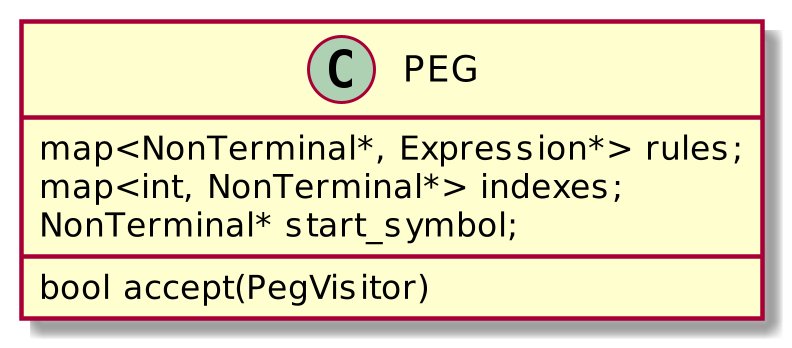
\includegraphics[width=0.50\textwidth]{uml/peg}
	\caption{Μοντελοποίηση μίας PEG}
    \label{fig:peg}
\end{figure}

\begin{minipage}{\textwidth}

Επομένως, τα βασικά πεδία μίας PEG είναι τα εξής:

\begin{description}[font=$\bullet$\scshape\bfseries]
	\item rules: Οι κανόνες θεωρούμε ότι είναι μία αντιστοίχιση από μη τερματικά σε σύνθετες εκφράσεις
	\item indexes: Η γραμματική ενσωματώνει την πληροφορία για την αντιστοιχία των μη τερματικών με μοναδικούς ακεραίους.
	\item start\_symbol: Το αρχικό σύμβολο της γραμματικής
\end{description}

\end{minipage}

\vspace{0.5cm}
Όπως και τα επιμέρους στοιχεία της, η γραμματική δέχεται έναν visitor.

\subsection{Υλοποίηση του συντακτικού αναλυτή}

Αφού μοντελοποιήσαμε μία PEG, μπορούμε τώρα να κάνουμε το ίδιο και για έναν συντακτικό αναλυτή για αυτήν. 
Πώς όμως θα μοντελοποιήσουμε έναν τέτοιο συντακτικό αναλυτή?
Είπαμε προηγουμένως ότι μία γραμματική PEG θα δέχεται έναν τέτοιον αναλυτή ως επισκέπτη (visitor).
Επιπλέον, ο parser μας πρέπει να ενθυλακώσει (encapsulate):

\begin{description}[font=$\bullet$\scshape\bfseries]
	\item Τη συμβολοσειρά εισόδου
	\item Την τρέχουσα θέση όπου βρίσκεται η ανάλυση στη συμβολοσειρά εισόδου
	\item Τον πίνακα ενδιάμεσων αποτελεσμάτων
	\item Τη δυνατότητα να αναλύσει συντακτικά μία PEG, καθώς και τα μεμονωμένα συστατικά της
\end{description}

Με βάση τα παραπάνω, μια μοντελοποίηση για τον Packrat Parser θα ήταν η εξής:

\begin{figure}[h]
    \centering
	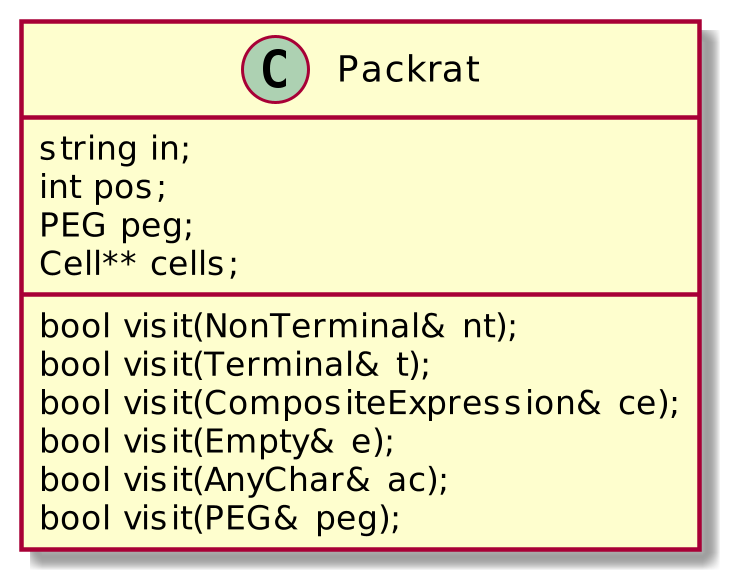
\includegraphics[width=0.50\textwidth]{uml/packrat}
	\caption{Μοντελοποίηση του Packrat Parser}
    \label{fig:packrat_parser}
\end{figure}

\newpage
Παρατηρούμε ότι, αντίστοιχα με μία PEG και τα συστατικά της που δέχονται ως "επισκέπτη" έναν συντακτικό αναλυτή, ο Packrat Parser υλοποιεί τις μεθόδους του επισκέπτη (visitor pattern).
Περισσότερα σχετικά με τα πλεονεκτήματα και μειονεκτήματα του Packrat Parsing, ιδιαίτερα σε σχέση με τις Context Free Grammars μπορούν να βρεθούν στο \cite{Ford2004}.

Ενδεικτικά, η μέθοδος \textit{visit(NonTerminal\& nt)}, φαίνεται στο Σχήμα \ref{fig:visit_nt}:

\begin{figure}[h]
\setlength\partopsep{-\topsep}% adjusts vertical space after the listing
\begin{minted}[frame=lines,linenos,numbersep=5pt]{c++}
bool SerialPackrat::visit(NonTerminal& nt)
{
    int row = nt.index();
    Cell* cur_cell = &cells[row][pos];
    Result cur_res = cur_cell->res();

    switch (cur_res) {

        case Result::success:
        {
            pos = cur_cell->pos();
            return true;
        }
        case Result::fail:
        {
            return false;
        }
        case Result::unknown:
        {
            Expression* e = peg.get_expr(&nt);
            auto res = e->accept(*this);

            if (res) {
                cur_cell->set_res(Result::success);
                cur_cell->set_pos(pos); // pos has changed
                return true;
            } else {
                cur_cell->set_res(Result::fail);
                return false;
            }
        }
    }
    return false;
}
\end{minted}
  \caption{Συντακτική ανάλυση ενός μη τερματικού}
  \label{fig:visit_nt}
\end{figure}

Αρχικά βρίσκουμε σε ποιο κελί του πίνακα αντιστοιχεί το μη τερματικό, με βάση το μοναδικό αριθμό του τερματικού (για τη γραμμή του πίνακα) και με βάση τη τρέχουσα θέση εισόδου (για τη στήλη του πίνακα) (γραμμές 3-5).
Στη συνέχεια, αν το ενδιάμεσο αποτέλεσμα είναι ήδη υπολογισμένο, επιστρέφουμε ανάλογα με την περίπτωση είτε επιτυχώς, θέτοντας την αντίστοιχη θέση στην είσοδο (γρ. 9-13), είτε ανεπιτυχώς (γρ. 14-17).
Αλλιώς, το υπολογίζουμε και αποθηκεύουμε το αντίστοιχο ενδιάμεσο αποτέλεσμα (γρ. 18-31).

Επιπλέον, η μέθοδος \textit{visit(Terminal\& t)}, φαίνεται στο Σχήμα \ref{fig:visit_t}:

\begin{figure}[h]
\setlength\partopsep{-\topsep}% adjusts vertical space after the listing
\begin{minted}[frame=lines,linenos,numbersep=5pt]{c++}
bool SerialPackrat::visit(Terminal& t)
{
    int terminal_char = t.name()[0];
    ...
    if (pos < in.size() && terminal_char == this->cur_tok()) {
        pos++;
        return true;
    }
    return false;
}
\end{minted}
  \caption{Συντακτική ανάλυση ενός τερματικού}
  \label{fig:visit_t}
\end{figure}

Πρακτικά, ο αναλυτής κοιτάει αν ο χαρακτήρας στο τρέχον σημείο εισόδου ταυτίζεται με το χαρακτήρα του τερματικού.
Αν ναι, τότε επιστρέφει επιτυχώς και ανεβάζει κατά 1 το δείκτη της εισόδου.
Αλλιώς, επιστρέφει ανεπιτυχώς.

Τέλος, η μέθοδος \textit{visit(CompositeExpression\& t)}, φαίνεται στο Σχήμα \ref{fig:visit_ce} για την περίπτωση της ακολουθίας και της διατεταγμένης επιλογής:

\begin{figure}[h]
\setlength\partopsep{-\topsep}% adjusts vertical space after the listing
\begin{minted}[frame=lines,linenos,numbersep=5pt]{c++}
bool SerialPackrat::visit(CompositeExpression& ce)
{
    char op = ce.op_name();
    std::vector<Expression*> exprs = ce.expr_list();
    int orig_pos = pos;

    switch (op) {

        case '\b':  // sequence
        {
            for (auto expr : exprs)
                if (!expr->accept(*this)) {
                    pos = orig_pos;
                    return false;
                }
            return true;
        }
        case '/':   // ordered choice
        {
            for (auto expr : exprs) {
                pos = orig_pos;
                if (expr->accept(*this))
                    return true;
            }
            pos = orig_pos;
            return false;
        }
        ...
    }
}
\end{minted}
  \caption{Συντακτική ανάλυση της ακολουθίας και της διατεταγμένης επιλογής}
  \label{fig:visit_ce}
\end{figure}

Προκειμένου να διαχωρίσει μεταξύ των διάφορων σύνθετων εκφράσεων, ο συντακτικός αναλυτής κοιτάει τον τελεστή της σύνθετης έκφρασης, ο οποίος ανάλογα με τη σύμβαση υποδηλώνει και κάτι διαφορετικό (π.χ. ο χαρακτήρας '/' αντιστοιχεί στη διατεταγμένη επιλογή).

Για την ακολουθία, ο αναλυτής εξετάζει όλες τις υποεκφράσεις και, αν έστω και μία αποτύχει, θέτει το δείκτη εισόδου στην αρχική θέση και επιστρέφει ανεπιτυχώς.
Αλλιώς, αν πετύχουν όλες, επιστρέφει επιτυχώς (ο δείκτης εισόδου θα έχει προχωρήσει από τις εσωτερικές κλήσεις στις υποεκφράσεις).

Η δυαδική διαδικασία είναι στη διατεταγμένη επιλογή: ο αναλυτής κοιτάει μία μία τις υποεκφράσεις και, αν έστω και μία πετύχει, επιστρέφει επιτυχώς (με την πρώτη που πετυχαίνει, που θα έχει προχωρήσει αυτή το δείκτη εισόδου).
Αλλιώς, αν όλες αποτύχουν, επαναφέρει το δείκτη εισόδου και επιστρέφει ανεπιτυχώς.
